\documentclass{article}
\setlength{\parindent}{0in}
\usepackage[
bottom = 2.50cm,
left   = 2.50cm,
right  = 2.50cm]{geometry}
\newcommand{\code}{\texttt}

\usepackage{graphicx}% Include fig. files
\usepackage{dcolumn}% Align table columns on decimal point
\usepackage{bm}% bold math
\usepackage{caption}
\usepackage[labelformat=simple]{subcaption}
\usepackage{float}
\usepackage{amsmath}
\usepackage{amssymb}
\usepackage[export]{adjustbox}
\usepackage[dvipsnames]{xcolor}
\usepackage{authblk}
\usepackage{url}
\usepackage{listings}
\usepackage{braket}

\begin{document}

\title{ESC407 Lab 1}

\author{Maggie Wang}

\date{October 2, 2023}
\maketitle

\begin{enumerate}
\item Central Differences for Numerical Differentiation
\begin{enumerate}
    \item The derivative of $f(x)=e^{2x}$ was calculated numerically at $x=0$, using central differences. 
    Table \ref{tab:1a} lists the numerically computed value of $f'(0)$ for different step sizes $h$ between $10^{-16}$ and $1$.
    
    \begin{table}[h]
        \centering
        \begin{tabular}{c|c c c c c c}
            $h$ & $10^{-16}$ & $10^{-15}$ & $10^{-14}$ & $10^{-13}$ & 
            $10^{-12}$ \\ 
            $f'(0)$ & 1.11022302 & 2.10942375 & 1.99840144 & 1.99951167 &
            2.00006678 \\  [0.2 em] \hline  \\[-0.8em]
            $h$ & $10^{-11}$ & $10^{-10}$ & $10^{-9}$ & $10^{-8}$ & 
            $10^{-7}$ & $10^{-6}$ \\ 
            $f'(0)$ & 2.00000017 & 2.00000017 & 2.00000005 & 1.99999999 & 2. & 2. \\ [0.2 em] \hline  \\[-0.8em]
            $h$ & $10^{-5}$ & $10^{-4}$ & $10^{-3}$ & $10^{-2}$ & $10^{-1}$ & $10^{0}$\\
            $f'(0)$  & 2. & 2. & 2.00000033 & 2.00003333 & 2.003335 & 2.35040239
        \end{tabular}
        \caption{Derivative of $f(x)=e^{2x}$ at $x=0$ for different $h$ values}
        \label{tab:1a}
    \end{table}

    The raw output from the code is 
    \begin{verbatim}
1 a) errors:  [1.11022302 2.10942375 1.99840144 1.99951167 2.00006678 2.00000017
2.00000017 2.00000005 1.99999999 2.         2.         2.
2.         2.00000033 2.00003333 2.003335   2.35040239]
    \end{verbatim}

    \item The minimum in error and the corresponding step size matches the expected value, calculated using $C=10^{-16}$. 
    The calculated error as a function of $h$ is shown in fig \ref{fig:1b}. The estimated optimal step size is $6.7\times 10^{-6}$, with a corresponding error of $4.48\times 10^{-11}$. 
    \begin{figure}[h]
        \centering 
        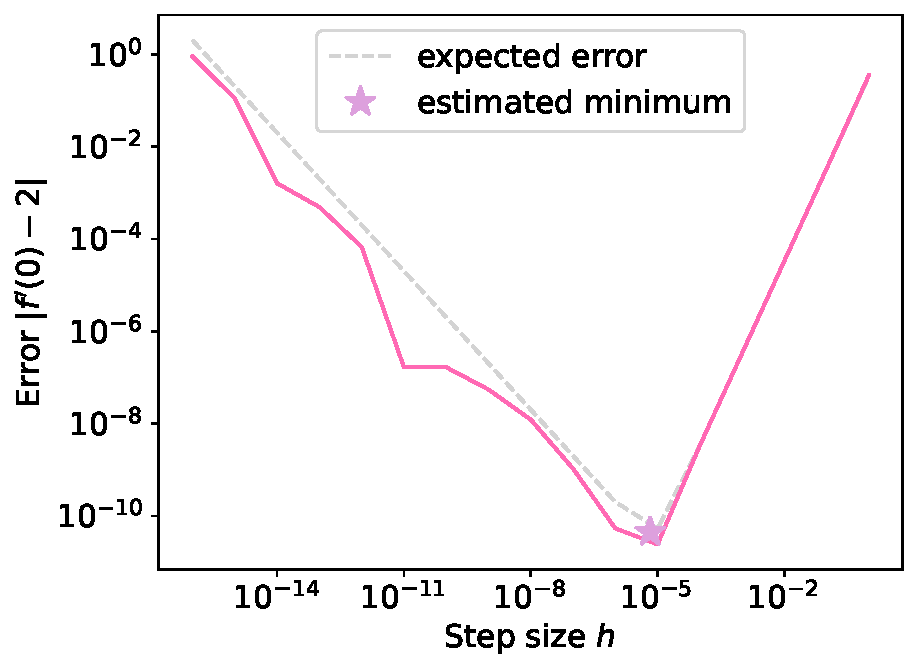
\includegraphics[width=0.48\textwidth]{Q1b.pdf}
        \caption{Calculated error vs $h$}
        \label{fig:1b}
      \end{figure}

    \item The first 10 derivatives of $f'(x)$ at $x=0$ calculated using central differences with the optimal step size (which is the same for all derivatives of $f(x)$)
    are listed in table \ref{tab:1c}.
    \begin{table}[h]
        \centering
        \begin{tabular}{c|c c c c c}
            $m$ & 1 & 2 & 3 & 4 & 5 \\
            $f'(0)$ & 2 & 4 & 7.77 & -2.21$\times 10^5$ & 8.26$\times 10^9$ \\ [0.2 em] \hline  \\[-0.8em]
            & 6 & 7 & 8 & 9 & 10\\
            & 2.22$\times 10^{16}$ & -3.69$\times 10^{20}$ & -2.12$\times 10^{27}$ & 2.06$\times 10^{31}$ & 2.0$\times 10^{38}$
        \end{tabular}
        \caption{Approximate values for $f^m(0)$ computed using central differences}
        \label{tab:1c}
    \end{table}
    The raw output from the code is:
\begin{verbatim}
1 c) derivatives:  [2.0000000000234888, 4.000001933007014, 7.77155789571232, 
    -221126.08039335813, 8258210993.557659, 2.2204420456714464e+16, 
    -3.68559504405105e+20, -2.1195518363153336e+27, 2.05607099203305e+31, 
    1.971716534777767e+38]
\end{verbatim}
\end{enumerate}

\item Integrating the Dawson Function Again
\begin{enumerate}
  \item Fig \ref{fig:2a} shows the Dawson function at $x=4$ evaluated using trapezoidal rule, Simpson's rule and gaussian quadrature for varying integration slices $N$. 
  The function calculated using gaussian quadrature converges much more quickly than integration schemes using Newton-Cotes formulae.
  \begin{figure}[h]
    \centering 
    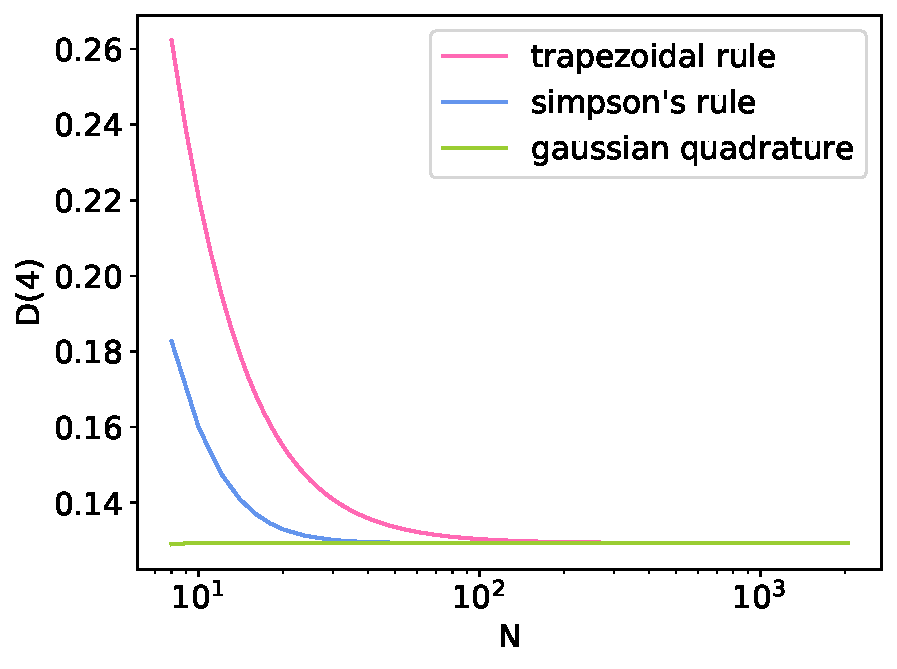
\includegraphics[width=0.4\textwidth]{Q2a.pdf}
    \caption{Dawson function $D(x)$ at $x=4$ calculated numerically vs number of integration slices $N$}
    \label{fig:2a}
  \end{figure}

  \item The error on $D(4)$ using gaussian quadrature, $I_{2N} - I_N$ for the values of $N$ in 2a) are plotted in fig \ref{fig:2b}. The error decreases quickly from $N=8$ to around $N=20$, and then remains around the machine precision limit.
  \begin{figure}[h]
    \centering 
    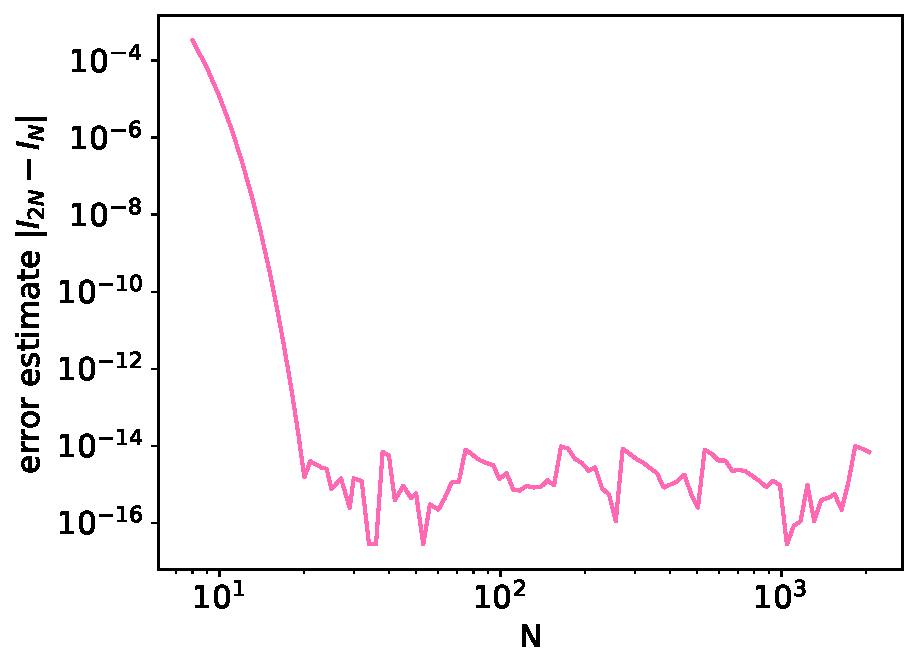
\includegraphics[width=0.42\textwidth]{Q2b.pdf}
    \caption{Error on $D(4)$ using gaussian quadrature vs number of integration slices}
    \label{fig:2b}
  \end{figure}
  \item Fig \ref{fig:2c} shows the relative error on $D(4)$ calculated using gaussian quadrature compared to the true value (from Scipy) as a function of the number of integration slices. 
  The behaviour of the relative error is the same as the estimated error from fig \ref{fig:2b}, while being around an order or magnitude larger than the estimated error.
  \begin{figure}[H]
    \centering 
    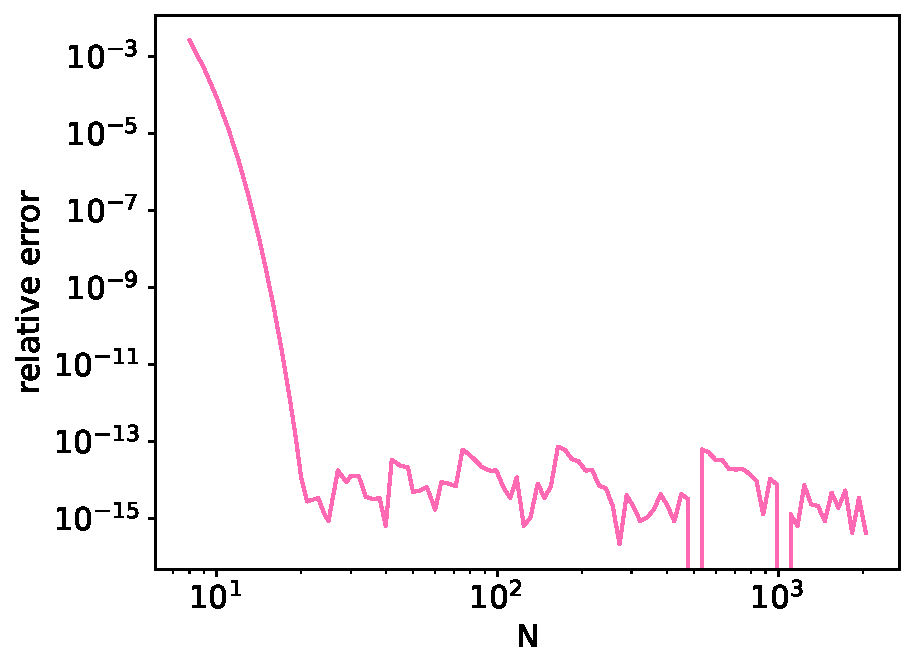
\includegraphics[width=0.42\textwidth]{Q2c.pdf}
    \caption{Relative error on $D(4)$ vs number of integration slices}
    \label{fig:2c}
  \end{figure}

\end{enumerate}

\item Calculating potential energy of QM harmonic oscillator 
\begin{enumerate}
    \item A function $H(n, x)$ was written to calculate the $n^{th}$ degree Hermite polynomial for a given x based on its recursion relation
    $H_{n+1}(x) = 2xH_n(x)-2nH_{n-1}(x)$.

    \item Fig \ref{fig:3b} shows the wave functions for the first 4 energy levels of a 1D quantum harmoniz oscillator.
    \begin{figure}[H]
        \centering 
        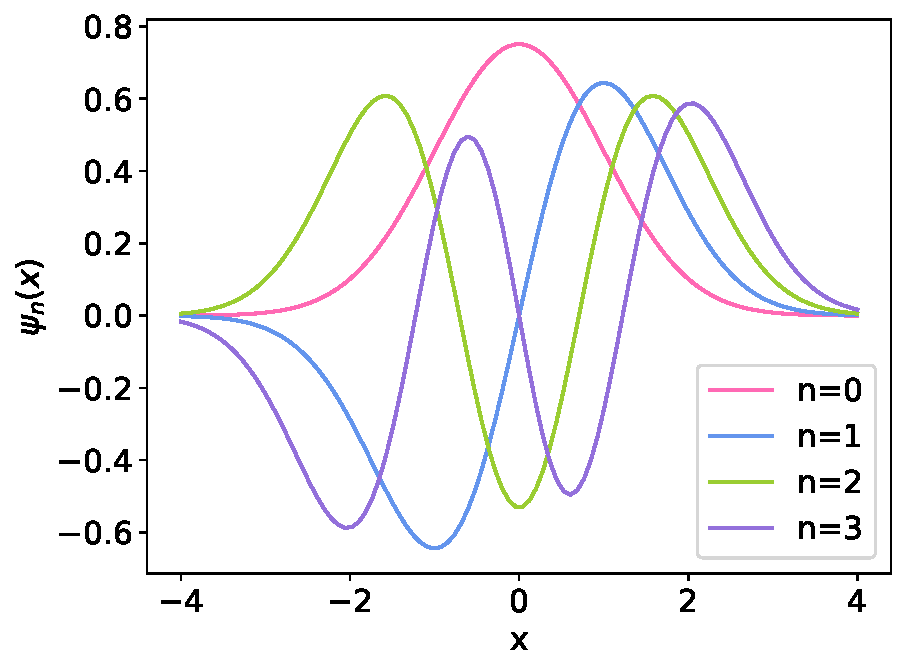
\includegraphics[width=0.42\textwidth]{Q3b.pdf}
        \caption{Harmonic oscillator wave functions}
        \label{fig:3b}
      \end{figure}

    \item The potential energy for $n$ from 0 to 10 computed using Gaussian quadrature using 100 points, from the formula 
    \begin{align*}
        PE &= \frac{\braket{x^2}}{2} = \int_{-\infty}^{\infty}x^2|\psi_n(x)|^2 dx
    \end{align*}
    The improper integral is calculated using the following transformation
    \begin{align*}
        \int_{-\infty}^{\infty} f(x) dx &= \int_{-\pi/2}^{\pi/2} \frac{f(\text{tan }z)}{\text{cos}^2 z} dz
    \end{align*}
    The potential energies are listed in table \ref{tab:3c}
    \begin{table}[h]
        \centering
        \begin{tabular}{c|c c c c c c c c c c c}
            $n$ & 0 & 1 & 2 & 3 & 4 & 5 & 6 & 7 & 8 & 9 & 10 \\
            $\braket{x^2}$ & 0.25 & 0.75 & 1.25 & 1.75 & 2.25 & 2.75 & 3.25 & 3.75 & 4.25 & 4.75 & 5.25
        \end{tabular}
        \caption{Potential energies of the quantum harmonic oscillator}
        \label{tab:3c}
    \end{table}

    The raw output from the code is 
\begin{verbatim}
0 0.24999999999999997
1 0.7500000000000119
2 1.2500000000003055
3 1.7499999999981126
4 2.249999999916142
5 2.7499999996902913
6 3.250000005587624
7 3.750000044358483
8 4.249999920351134
9 4.749998195042198
10 5.24999677662962
\end{verbatim}
\end{enumerate}

\end{enumerate}


\end{document}